\scanpage{6}
\mspage{5}
commute à tt changement de base $Y'-Y$.

\uline{NB} Vrai sans hyp. de propreté si $Y'\to Y$ est \uline{lisse}, $f$ qu. cpt. qu. sép., et $F$ premier aux car. rés. de $Y$.

\deleted{\unsure{8°)} \uline{Ex} Morphisme fini $R^qf_*(F)=0\quad q\ne0$}

\figure{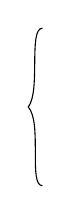
\begin{tikzpicture}\draw (.18,1) .. controls (0,1) and (.16,.2) .. (0,0) .. controls (.18,-.2) and (0,-1) .. (.18,-1);\end{tikzpicture}}
\uline{Ex}
\[
R^qf_*(F)_{\bar y}\simeq H^q(X_{\bar y},F_{\bar y})
\]
\uline{Ex.} $X$ \inserted{prop.} sur $k$ sép. clos, $k'$ ext. sép. clos de $k$, d'où $X'=X_{k'}$, $F'=F_{X'}$, et $H^i(X,F)\simeq H^i(X',F')$.

\uline{NB} Vrai sans hyp. de propreté si $F$ de torsion \unsure{première} à \deleted{\unsure{la car.}} $\operatorname{car} k$.

8°) \uline{Comparaison avec la cohomologie classique}

$X$ \unsure{préschéma} loc. alg. sur $\mathbf C$, alors pour tt $F$ faisceau de torsion sur $X$,
\[
H^q(X,F)\longrightarrow H^q(X^{\mathrm{tr}},F^{\mathrm{tr}})
\]
est un \uline{isomorphisme}. Résultat analogue pour un morphisme $f:X\longrightarrow Y$, si $f$ est \deleted{propre} \uline{de type fini}.

\margin{Utilise en plus résolution \unsure{sing.} \unsure{si on fait|sauf} \deleted{\unsure{avec}} l'hyp de propreté.}

\margin{\uline{Gaga} plus complet : OK. pour \deleted{\unsure{Hom}} \unsure{Ét} \unsure{les} faisceaux de torsion : équivalence de catégories des faisceaux constructibles algébriques et faisceaux constructibles analytiques qui sont \uline{de torsion}. \unsure{à rédiger} .....}

\deleted{\uline{Remarque} Soit $X$ un schéma propre sur un \unsure{anneau} analytique \inserted{$A=\mathcal O_{Y,y}$} sur $\mathbf C$, i.e. $Y$ un \unsure{espace} analytique sur $\mathbf C$. Alors $X$ ``provient'' d'un \unsure{schéma} analytique $X'$ \uline{propre} au dessus d'un voisinage ouvert $Y'$ de $Y$. \deleted{\unsure{A pour un faisceau}} tt faisceau \inserted{de torsion} constr. $F'$ sur $X'$ ``induit'' un \deleted{\unsure{faisceau}} constr. $F$ sur $X$.}
